\section[ad]{Adversarial networks / Generative Models}

\begin{frame}
  \frametitle{Generative Adversarial Network}
    \begin{center}
      \begin{tikzpicture}[scale=0.5]

        \draw (-3,1) rectangle (-2.5,0.5);
        \draw (-3,0.5) rectangle (-2.5,0);
        \draw (-3,0) rectangle (-2.5,-0.5);
        \draw (-3,-0.5) rectangle (-2.5,-1);
        \draw (-3,-1) rectangle (-2.5,-1.5);
        \draw (-3,-1.5) rectangle (-2.5,-2);
        \draw (-3,-2) rectangle (-2.5,-2.5);
        \draw (-3,-2.5) rectangle (-2.5,-3);
    
        \node[anchor=center] at (2,1.5) {\small Generative Neural Network};
        \begin{scope}
        \clip[rounded corners=2ex] (0,1) rectangle (4,-3);
          \node[anchor=center,inner sep=0]  at (2, -1) {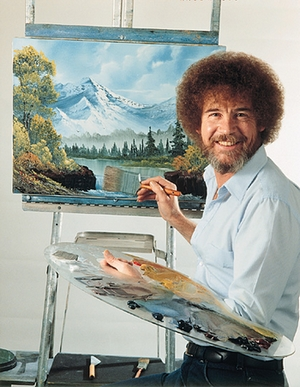
\includegraphics[height=0.4\textheight]{BobRoss.jpg}};
        \end{scope}

        \node[anchor=center] at (2,-4.5) {\small Photographs};
        \begin{scope}
        \clip[rounded corners=2ex] (0,-5) rectangle (4,-9);
          \node[anchor=center,inner sep=0]  at (2, -7) {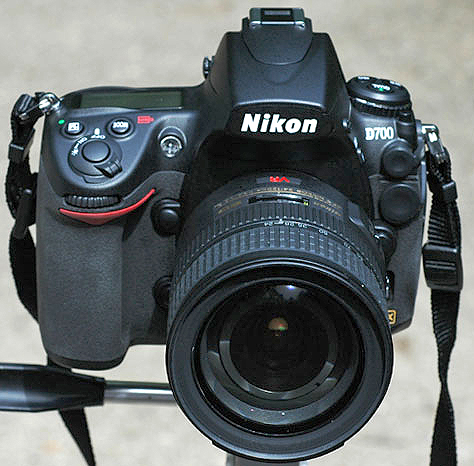
\includegraphics[height=0.4\textheight]{foto.jpg}};
        \end{scope}
    
        \node[anchor=center] at (10,-1.5) {\small Adversarial Neural Network};
        \begin{scope}
        \clip[rounded corners=2ex] (8,-2) rectangle (12,-6);
        \draw[rounded corners=2ex] (8,-2) rectangle (12,-6);
    
          \node[anchor=center,inner sep=0]  at (10, -4) {\small Fake or Real?};
        \end{scope}
    
        \draw[->, -latex', line width=0.05cm] (-2.3,-1) -- (-0.2,-1) node[sloped,below,midway] {\tiny White noise};
        \draw[->, -latex', line width=0.05cm] (4,-1) -- (8,-3.5) node[sloped,below,midway] {\tiny Fake images};
        \draw[->, -latex', line width=0.05cm] (4,-7) -- (8,-4.5) node[sloped,above,midway] {\tiny Real images};
      \end{tikzpicture}

    \begin{itemize}
      \item Generative network (G) learns to create images from random inputs
      \item Adversarial network (A) distinguishes fake and real images
      \item Adapt weights of G so that the loss of A is maximized
    \end{itemize}

    \end{center}
\end{frame}

\begin{frame}
\frametitle{Example: Arithmetic with Faces}
\begin{center}
      \begin{tikzpicture}
          \node[anchor=center,inner sep=0]  at (0, 0) {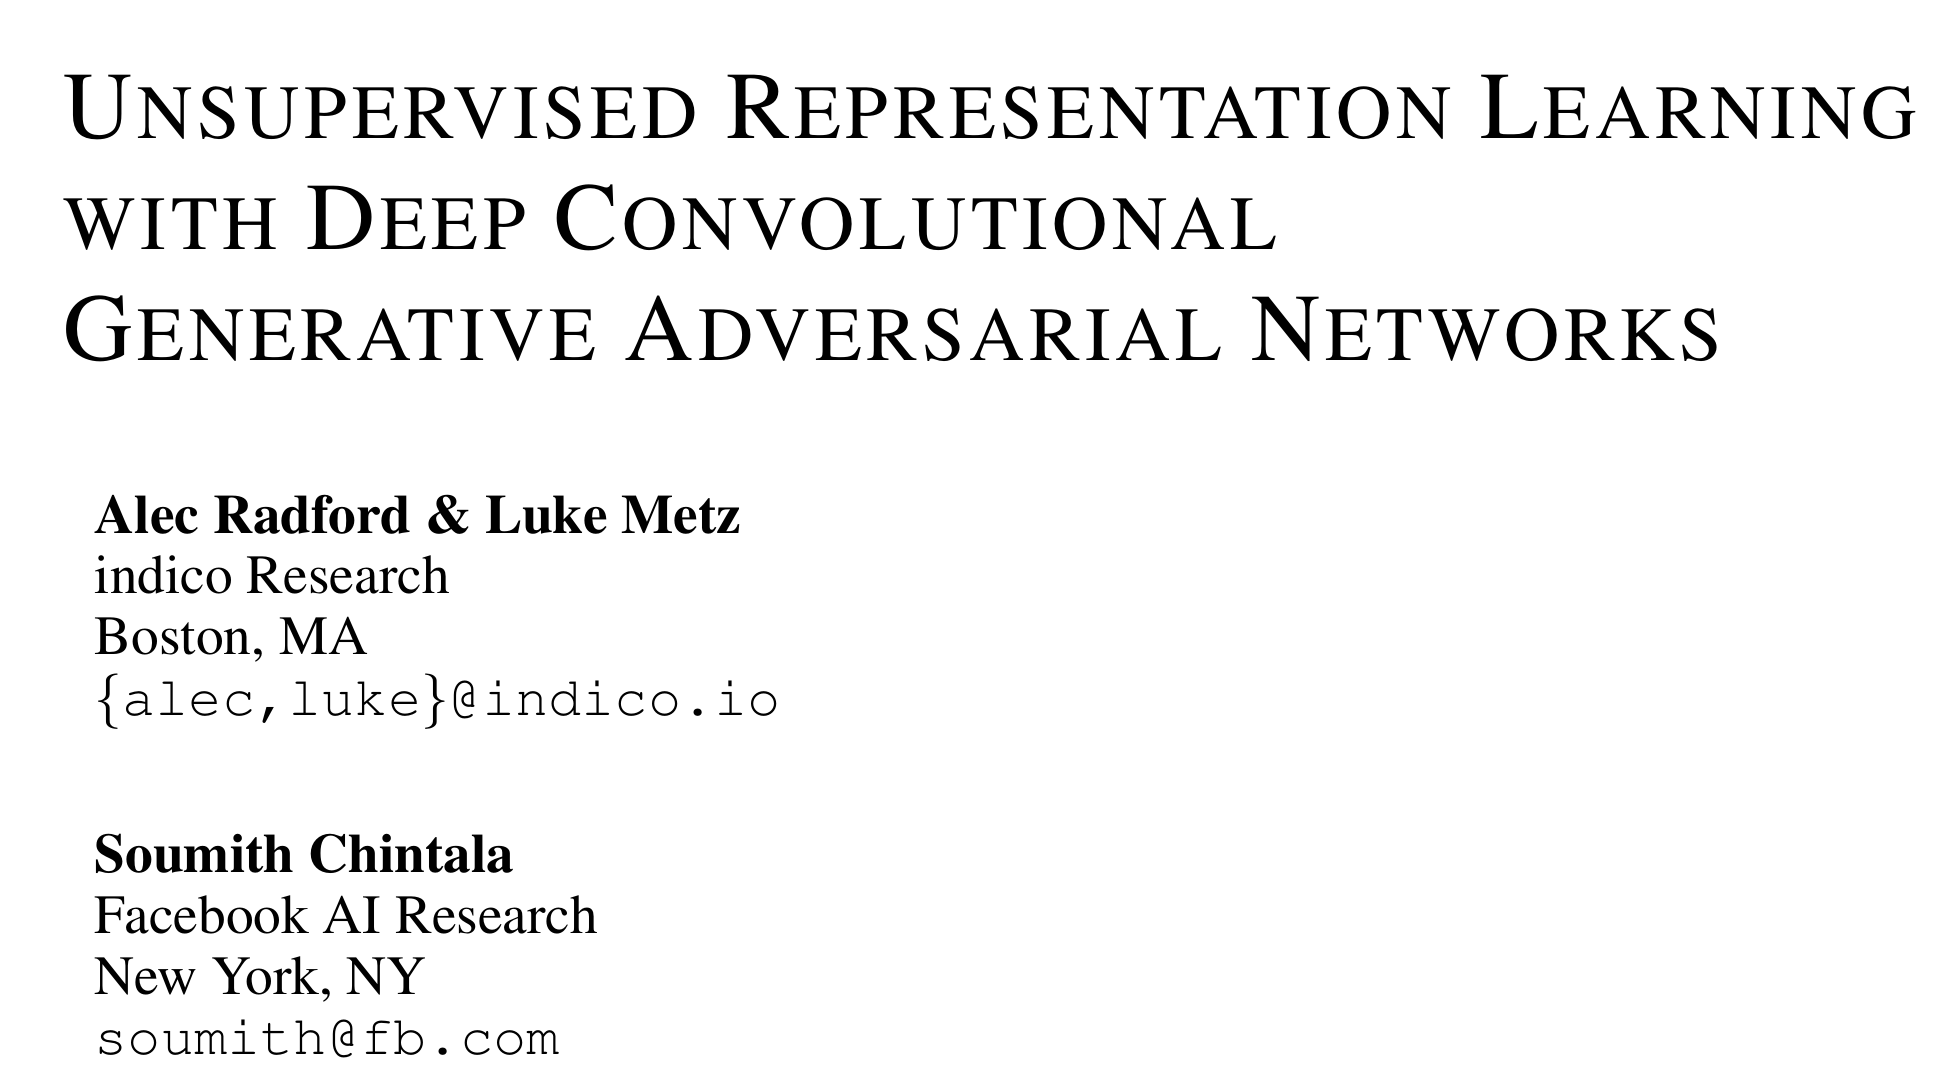
\includegraphics[height=0.4\textheight]{gan_paper.png}};
          \node[anchor=center,inner sep=0]  at (0, -3) {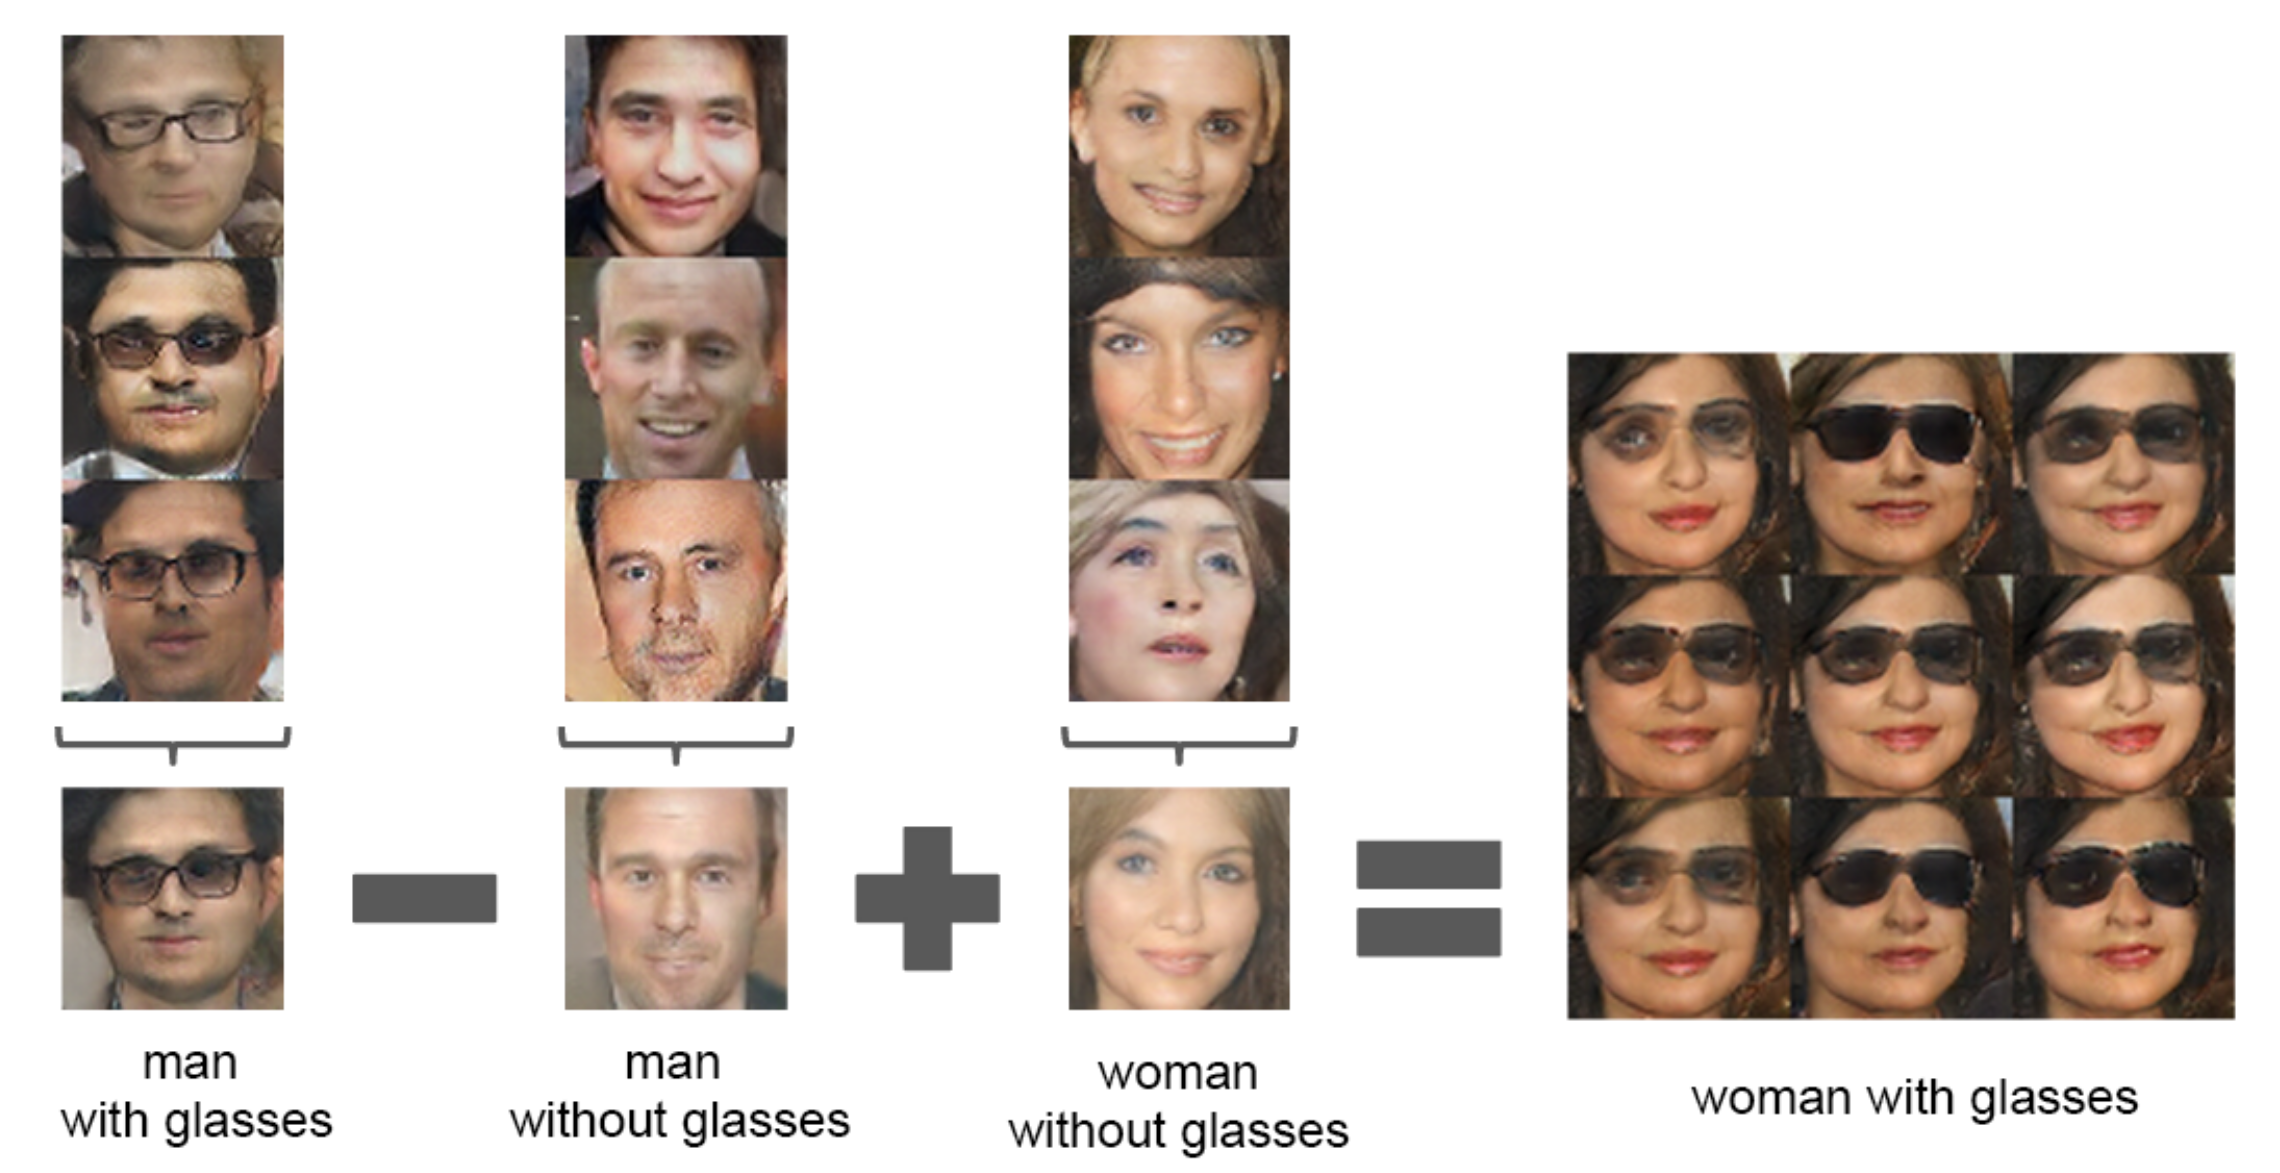
\includegraphics[width=0.7\textwidth]{gan_faces.png}};
      \end{tikzpicture}
      \end{center}
\end{frame}

\begin{frame}
\frametitle{Example: Learning to Pivot}
\begin{center}
      \begin{tikzpicture}
          \node[anchor=center,inner sep=0]  at (0, 0) {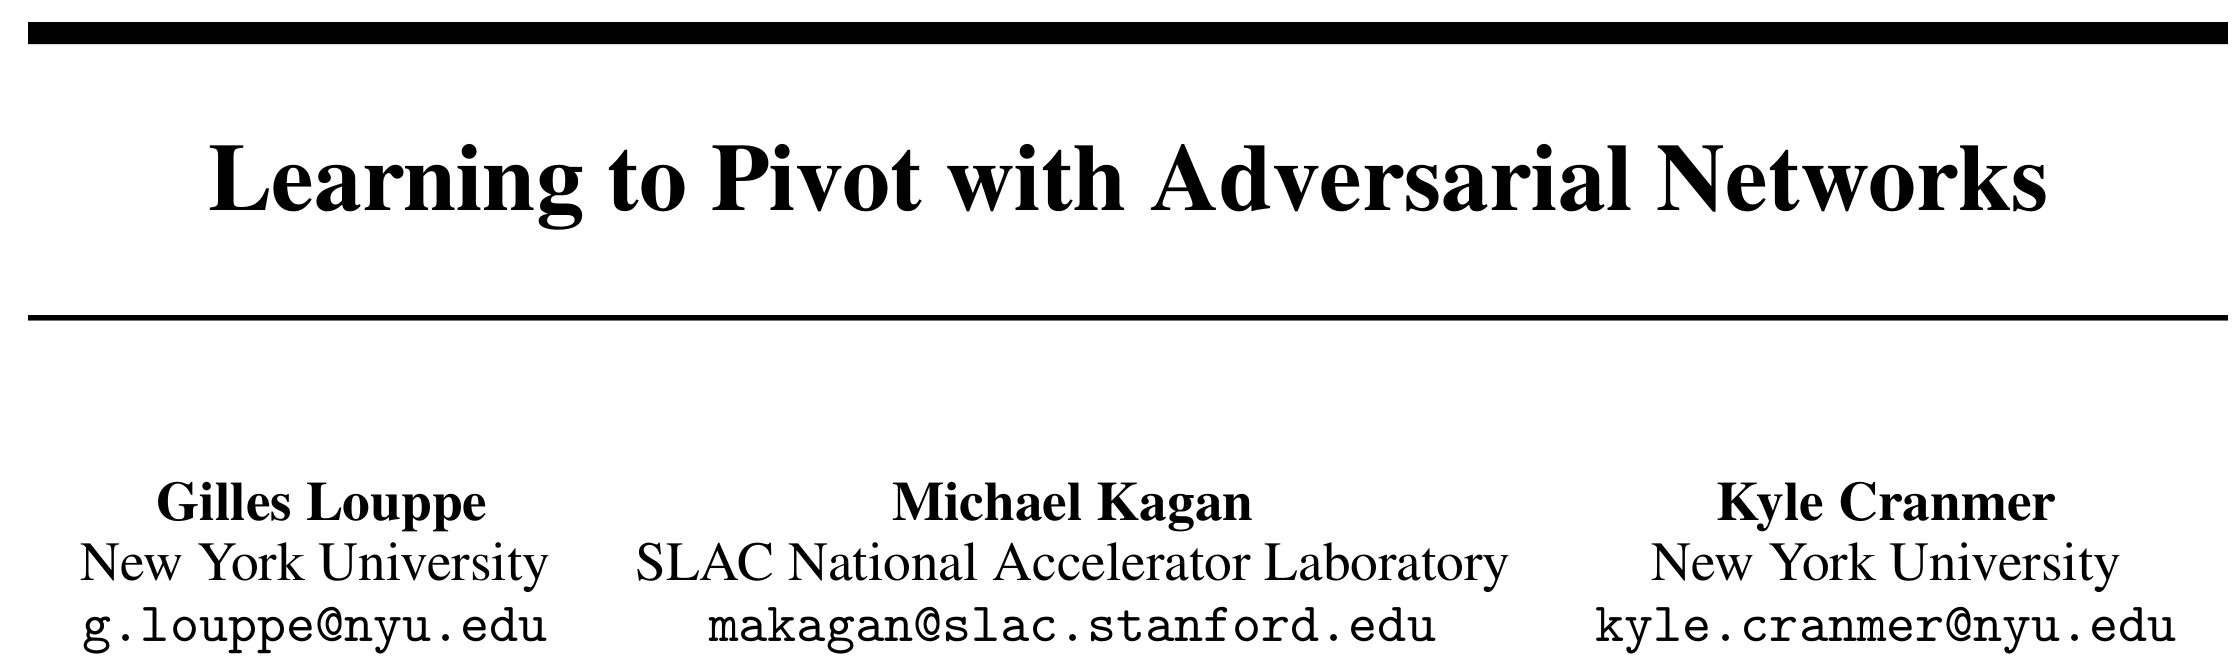
\includegraphics[height=0.2\textheight]{ltp_paper.png}};
          \node[anchor=center,inner sep=0]  at (0, -2.5) {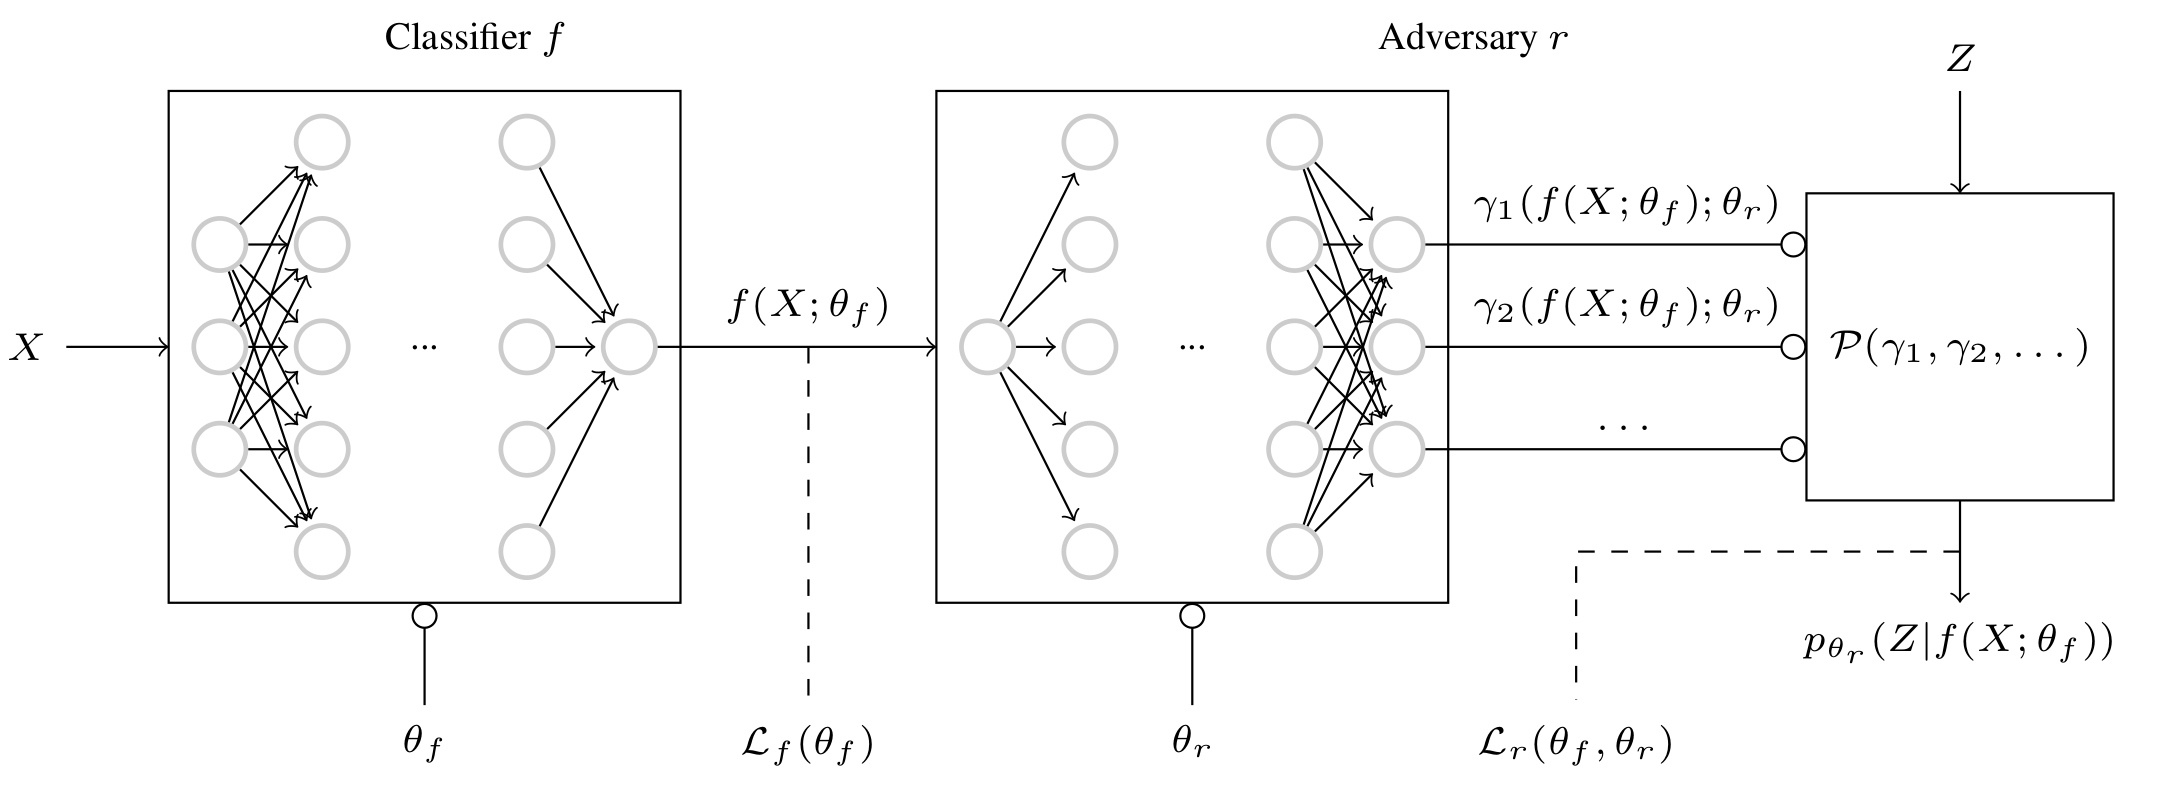
\includegraphics[height=0.3\textheight]{ltp_network.png}};
          \node[anchor=center,inner sep=0]  at (0, -5.5) {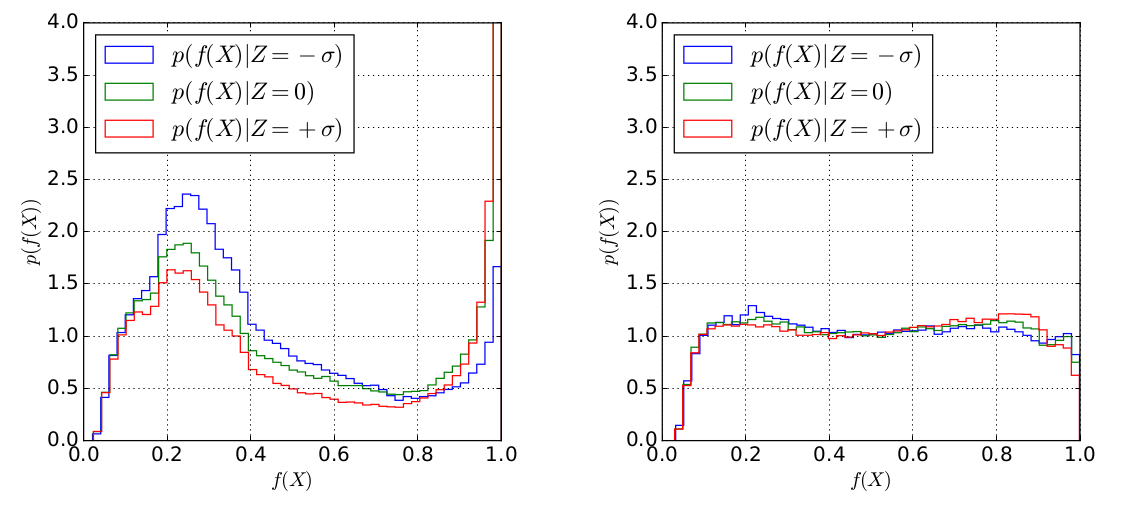
\includegraphics[height=0.3\textheight]{tlp_result.png}};
      \end{tikzpicture}
      \end{center}
\end{frame}

\begin{frame}
\frametitle{Aside: Adversarial Examples}
\begin{center}
\vspace{-1em}
      \begin{tikzpicture}
          \node[anchor=center,inner sep=0]  at (0, 0) {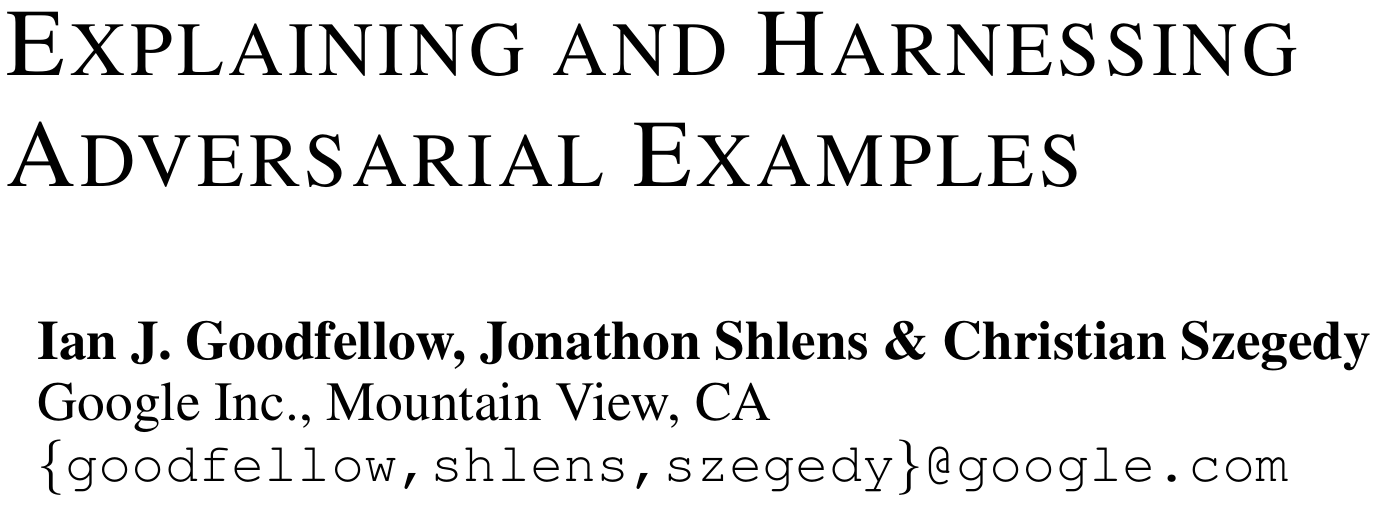
\includegraphics[height=0.15\textheight]{adversarial_paper.png}};
          \node[anchor=center,inner sep=0]  at (0, -2.8) {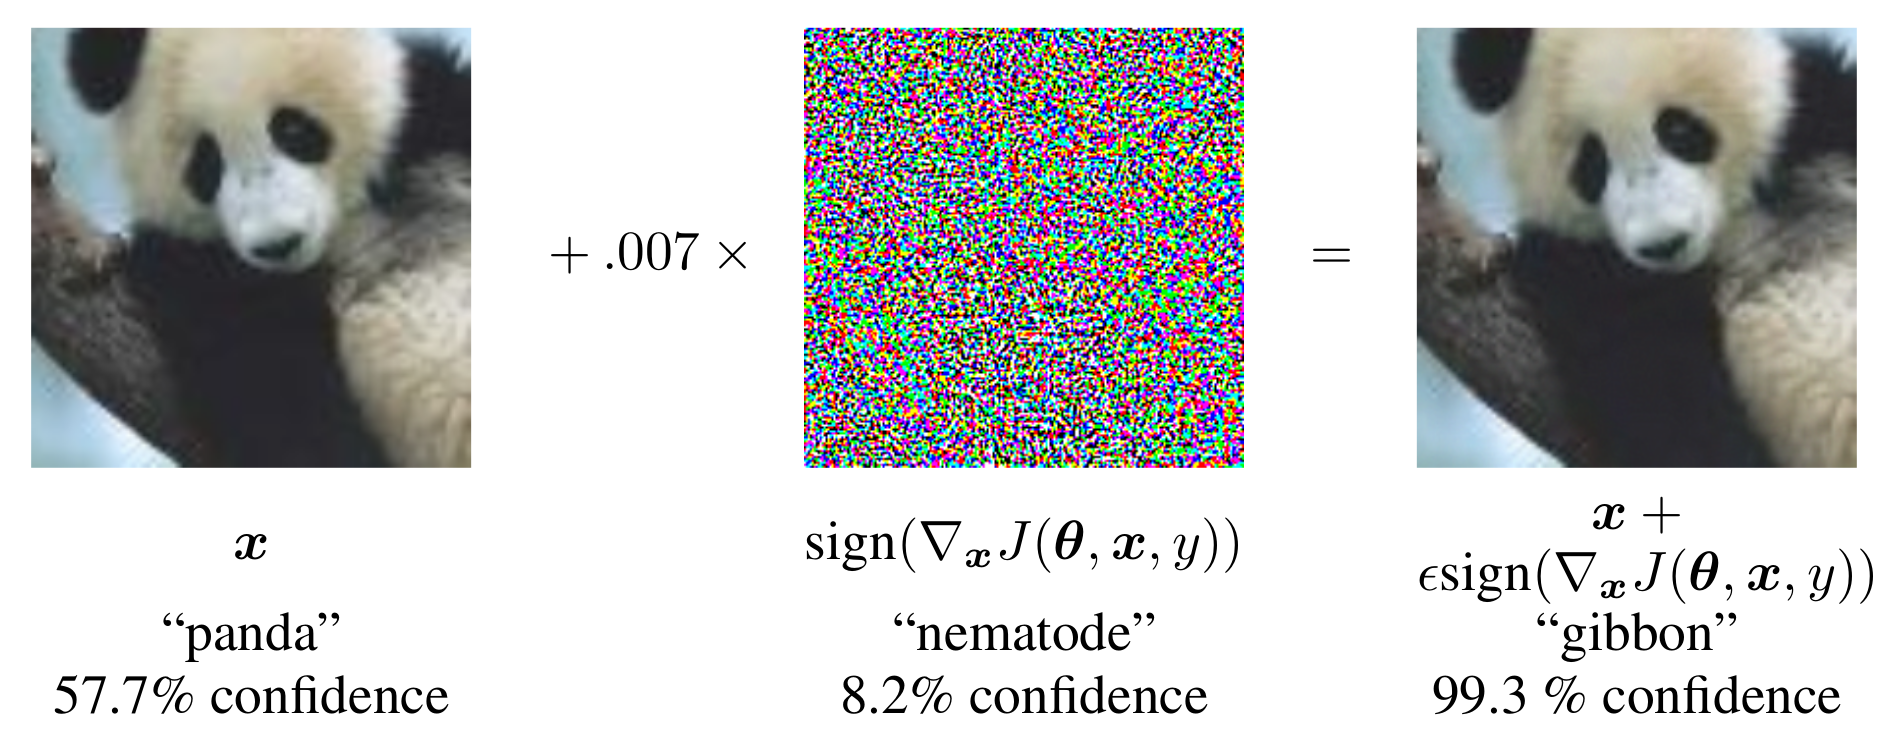
\includegraphics[height=0.4\textheight]{adversarial_example.png}};
      \end{tikzpicture}
      \end{center}
      \textbf{Idea: Add noise to introduce shifts in the network output}
      
      \begin{quote}
      Adversarial examples [...] are a result of models being too linear, rather than too nonlinear. -- I. Goodfellow et. al.
      \end{quote}
\end{frame}

\begin{frame}
\frametitle{Aside: Adversarial Training}
\begin{center}
	\textbf{Idea}
	\begin{itemize}
	\item Train on original and adversarial examples
	\item Generate adversarial examples on-the-fly in the loss-function $\mathcal{J}$
	\end{itemize}
	
	\begin{align*}
	\tilde{\mathcal{J}}(\vec{x}, t, \vec{\Theta}) &= \mathcal{J}(\vec{x}, t, \vec{\Theta}) + \mathcal{J}(\vec{x} + \epsilon \mathrm{sign}(\nabla_x \mathcal{J}(\vec{x}, t, \vec{\Theta})), t, \vec{\Theta})
	\end{align*}
	
	\textbf{Mitigates the problem, but it does not disappear}
\end{center}
      
\end{frame}

